
%% bare_conf.tex
%% V1.3
%% 2007/01/11
%% by Michael Shell
%% See:
%% http://www.michaelshell.org/
%% for current contact information.
%%
%% This is a skeleton file demonstrating the use of IEEEtran.cls
%% (requires IEEEtran.cls version 1.7 or later) with an IEEE conference paper.
%%
%% Support sites:
%% http://www.michaelshell.org/tex/ieeetran/
%% http://www.ctan.org/tex-archive/macros/latex/contrib/IEEEtran/
%% and
%% http://www.ieee.org/

%%*************************************************************************
%% Legal Notice:
%% This code is offered as-is without any warranty either expressed or
%% implied; without even the implied warranty of MERCHANTABILITY or
%% FITNESS FOR A PARTICULAR PURPOSE!
%% User assumes all risk.
%% In no event shall IEEE or any contributor to this code be liable for
%% any damages or losses, including, but not limited to, incidental,
%% consequential, or any other damages, resulting from the use or misuse
%% of any information contained here.
%%
%% All comments are the opinions of their respective authors and are not
%% necessarily endorsed by the IEEE.
%%
%% This work is distributed under the LaTeX Project Public License (LPPL)
%% ( http://www.latex-project.org/ ) version 1.3, and may be freely used,
%% distributed and modified. A copy of the LPPL, version 1.3, is included
%% in the base LaTeX documentation of all distributions of LaTeX released
%% 2003/12/01 or later.
%% Retain all contribution notices and credits.
%% ** Modified files should be clearly indicated as such, including  **
%% ** renaming them and changing author support contact information. **
%%
%% File list of work: IEEEtran.cls, IEEEtran_HOWTO.pdf, bare_adv.tex,
%%                    bare_conf.tex, bare_jrnl.tex, bare_jrnl_compsoc.tex
%%*************************************************************************

% *** Authors should verify (and, if needed, correct) their LaTeX system  ***
% *** with the testflow diagnostic prior to trusting their LaTeX platform ***
% *** with production work. IEEE's font choices can trigger bugs that do  ***
% *** not appear when using other class files.                            ***
% The testflow support page is at:
% http://www.michaelshell.org/tex/testflow/



% Note that the a4paper option is mainly intended so that authors in
% countries using A4 can easily print to A4 and see how their papers will
% look in print - the typesetting of the document will not typically be
% affected with changes in paper size (but the bottom and side margins will).
% Use the testflow package mentioned above to verify correct handling of
% both paper sizes by the user's LaTeX system.
%
% Also note that the "draftcls" or "draftclsnofoot", not "draft", option
% should be used if it is desired that the figures are to be displayed in
% draft mode.
%
\documentclass[conference]{IEEEtran}
\usepackage{blindtext, graphicx}
% Add the compsoc option for Computer Society conferences.
%
% If IEEEtran.cls has not been installed into the LaTeX system files,
% manually specify the path to it like:
% \documentclass[conference]{../sty/IEEEtran}





% Some very useful LaTeX packages include:
% (uncomment the ones you want to load)


% *** MISC UTILITY PACKAGES ***
%
%\usepackage{ifpdf}
% Heiko Oberdiek's ifpdf.sty is very useful if you need conditional
% compilation based on whether the output is pdf or dvi.
% usage:
% \ifpdf
%   % pdf code
% \else
%   % dvi code
% \fi
% The latest version of ifpdf.sty can be obtained from:
% http://www.ctan.org/tex-archive/macros/latex/contrib/oberdiek/
% Also, note that IEEEtran.cls V1.7 and later provides a builtin
% \ifCLASSINFOpdf conditional that works the same way.
% When switching from latex to pdflatex and vice-versa, the compiler may
% have to be run twice to clear warning/error messages.






% *** CITATION PACKAGES ***
%
\usepackage{cite}
% cite.sty was written by Donald Arseneau
% V1.6 and later of IEEEtran pre-defines the format of the cite.sty package
% \cite{} output to follow that of IEEE. Loading the cite package will
% result in citation numbers being automatically sorted and properly
% "compressed/ranged". e.g., [1], [9], [2], [7], [5], [6] without using
% cite.sty will become [1], [2], [5]--[7], [9] using cite.sty. cite.sty's
% \cite will automatically add leading space, if needed. Use cite.sty's
% noadjust option (cite.sty V3.8 and later) if you want to turn this off.
% cite.sty is already installed on most LaTeX systems. Be sure and use
% version 4.0 (2003-05-27) and later if using hyperref.sty. cite.sty does
% not currently provide for hyperlinked citations.
% The latest version can be obtained at:
% http://www.ctan.org/tex-archive/macros/latex/contrib/cite/
% The documentation is contained in the cite.sty file itself.






% *** GRAPHICS RELATED PACKAGES ***
%
\ifCLASSINFOpdf
  % \usepackage[pdftex]{graphicx}
  % declare the path(s) where your graphic files are
  % \graphicspath{{../pdf/}{../jpeg/}}
  % and their extensions so you won't have to specify these with
  % every instance of \includegraphics
  % \DeclareGraphicsExtensions{.pdf,.jpeg,.png}
\else
  % or other class option (dvipsone, dvipdf, if not using dvips). graphicx
  % will default to the driver specified in the system graphics.cfg if no
  % driver is specified.
  % \usepackage[dvips]{graphicx}
  % declare the path(s) where your graphic files are
  % \graphicspath{{../eps/}}
  % and their extensions so you won't have to specify these with
  % every instance of \includegraphics
  % \DeclareGraphicsExtensions{.eps}
\fi
% graphicx was written by David Carlisle and Sebastian Rahtz. It is
% required if you want graphics, photos, etc. graphicx.sty is already
% installed on most LaTeX systems. The latest version and documentation can
% be obtained at:
% http://www.ctan.org/tex-archive/macros/latex/required/graphics/
% Another good source of documentation is "Using Imported Graphics in
% LaTeX2e" by Keith Reckdahl which can be found as epslatex.ps or
% epslatex.pdf at: http://www.ctan.org/tex-archive/info/
%
% latex, and pdflatex in dvi mode, support graphics in encapsulated
% postscript (.eps) format. pdflatex in pdf mode supports graphics
% in .pdf, .jpeg, .png and .mps (metapost) formats. Users should ensure
% that all non-photo figures use a vector format (.eps, .pdf, .mps) and
% not a bitmapped formats (.jpeg, .png). IEEE frowns on bitmapped formats
% which can result in "jaggedy"/blurry rendering of lines and letters as
% well as large increases in file sizes.
%
% You can find documentation about the pdfTeX application at:
% http://www.tug.org/applications/pdftex





% *** MATH PACKAGES ***
%
%\usepackage[cmex10]{amsmath}
% A popular package from the American Mathematical Society that provides
% many useful and powerful commands for dealing with mathematics. If using
% it, be sure to load this package with the cmex10 option to ensure that
% only type 1 fonts will utilized at all point sizes. Without this option,
% it is possible that some math symbols, particularly those within
% footnotes, will be rendered in bitmap form which will result in a
% document that can not be IEEE Xplore compliant!
%
% Also, note that the amsmath package sets \interdisplaylinepenalty to 10000
% thus preventing page breaks from occurring within multiline equations. Use:
%\interdisplaylinepenalty=2500
% after loading amsmath to restore such page breaks as IEEEtran.cls normally
% does. amsmath.sty is already installed on most LaTeX systems. The latest
% version and documentation can be obtained at:
% http://www.ctan.org/tex-archive/macros/latex/required/amslatex/math/





% *** SPECIALIZED LIST PACKAGES ***
%
%\usepackage{algorithmic}
% algorithmic.sty was written by Peter Williams and Rogerio Brito.
% This package provides an algorithmic environment fo describing algorithms.
% You can use the algorithmic environment in-text or within a figure
% environment to provide for a floating algorithm. Do NOT use the algorithm
% floating environment provided by algorithm.sty (by the same authors) or
% algorithm2e.sty (by Christophe Fiorio) as IEEE does not use dedicated
% algorithm float types and packages that provide these will not provide
% correct IEEE style captions. The latest version and documentation of
% algorithmic.sty can be obtained at:
% http://www.ctan.org/tex-archive/macros/latex/contrib/algorithms/
% There is also a support site at:
% http://algorithms.berlios.de/index.html
% Also of interest may be the (relatively newer and more customizable)
% algorithmicx.sty package by Szasz Janos:
% http://www.ctan.org/tex-archive/macros/latex/contrib/algorithmicx/




% *** ALIGNMENT PACKAGES ***
%
%\usepackage{array}
% Frank Mittelbach's and David Carlisle's array.sty patches and improves
% the standard LaTeX2e array and tabular environments to provide better
% appearance and additional user controls. As the default LaTeX2e table
% generation code is lacking to the point of almost being broken with
% respect to the quality of the end results, all users are strongly
% advised to use an enhanced (at the very least that provided by array.sty)
% set of table tools. array.sty is already installed on most systems. The
% latest version and documentation can be obtained at:
% http://www.ctan.org/tex-archive/macros/latex/required/tools/


%\usepackage{mdwmath}
%\usepackage{mdwtab}
% Also highly recommended is Mark Wooding's extremely powerful MDW tools,
% especially mdwmath.sty and mdwtab.sty which are used to format equations
% and tables, respectively. The MDWtools set is already installed on most
% LaTeX systems. The lastest version and documentation is available at:
% http://www.ctan.org/tex-archive/macros/latex/contrib/mdwtools/


% IEEEtran contains the IEEEeqnarray family of commands that can be used to
% generate multiline equations as well as matrices, tables, etc., of high
% quality.


%\usepackage{eqparbox}
% Also of notable interest is Scott Pakin's eqparbox package for creating
% (automatically sized) equal width boxes - aka "natural width parboxes".
% Available at:
% http://www.ctan.org/tex-archive/macros/latex/contrib/eqparbox/





% *** SUBFIGURE PACKAGES ***
%\usepackage[tight,footnotesize]{subfigure}
% subfigure.sty was written by Steven Douglas Cochran. This package makes it
% easy to put subfigures in your figures. e.g., "Figure 1a and 1b". For IEEE
% work, it is a good idea to load it with the tight package option to reduce
% the amount of white space around the subfigures. subfigure.sty is already
% installed on most LaTeX systems. The latest version and documentation can
% be obtained at:
% http://www.ctan.org/tex-archive/obsolete/macros/latex/contrib/subfigure/
% subfigure.sty has been superceeded by subfig.sty.



%\usepackage[caption=false]{caption}
%\usepackage[font=footnotesize]{subfig}
% subfig.sty, also written by Steven Douglas Cochran, is the modern
% replacement for subfigure.sty. However, subfig.sty requires and
% automatically loads Axel Sommerfeldt's caption.sty which will override
% IEEEtran.cls handling of captions and this will result in nonIEEE style
% figure/table captions. To prevent this problem, be sure and preload
% caption.sty with its "caption=false" package option. This is will preserve
% IEEEtran.cls handing of captions. Version 1.3 (2005/06/28) and later
% (recommended due to many improvements over 1.2) of subfig.sty supports
% the caption=false option directly:
%\usepackage[caption=false,font=footnotesize]{subfig}
%
% The latest version and documentation can be obtained at:
% http://www.ctan.org/tex-archive/macros/latex/contrib/subfig/
% The latest version and documentation of caption.sty can be obtained at:
% http://www.ctan.org/tex-archive/macros/latex/contrib/caption/




% *** FLOAT PACKAGES ***
%
%\usepackage{fixltx2e}
% fixltx2e, the successor to the earlier fix2col.sty, was written by
% Frank Mittelbach and David Carlisle. This package corrects a few problems
% in the LaTeX2e kernel, the most notable of which is that in current
% LaTeX2e releases, the ordering of single and double column floats is not
% guaranteed to be preserved. Thus, an unpatched LaTeX2e can allow a
% single column figure to be placed prior to an earlier double column
% figure. The latest version and documentation can be found at:
% http://www.ctan.org/tex-archive/macros/latex/base/



%\usepackage{stfloats}
% stfloats.sty was written by Sigitas Tolusis. This package gives LaTeX2e
% the ability to do double column floats at the bottom of the page as well
% as the top. (e.g., "\begin{figure*}[!b]" is not normally possible in
% LaTeX2e). It also provides a command:
%\fnbelowfloat
% to enable the placement of footnotes below bottom floats (the standard
% LaTeX2e kernel puts them above bottom floats). This is an invasive package
% which rewrites many portions of the LaTeX2e float routines. It may not work
% with other packages that modify the LaTeX2e float routines. The latest
% version and documentation can be obtained at:
% http://www.ctan.org/tex-archive/macros/latex/contrib/sttools/
% Documentation is contained in the stfloats.sty comments as well as in the
% presfull.pdf file. Do not use the stfloats baselinefloat ability as IEEE
% does not allow \baselineskip to stretch. Authors submitting work to the
% IEEE should note that IEEE rarely uses double column equations and
% that authors should try to avoid such use. Do not be tempted to use the
% cuted.sty or midfloat.sty packages (also by Sigitas Tolusis) as IEEE does
% not format its papers in such ways.





% *** PDF, URL AND HYPERLINK PACKAGES ***
%
%\usepackage{url}
% url.sty was written by Donald Arseneau. It provides better support for
% handling and breaking URLs. url.sty is already installed on most LaTeX
% systems. The latest version can be obtained at:
% http://www.ctan.org/tex-archive/macros/latex/contrib/misc/
% Read the url.sty source comments for usage information. Basically,
% \url{my_url_here}.





% *** Do not adjust lengths that control margins, column widths, etc. ***
% *** Do not use packages that alter fonts (such as pslatex).         ***
% There should be no need to do such things with IEEEtran.cls V1.6 and later.
% (Unless specifically asked to do so by the journal or conference you plan
% to submit to, of course. )


% correct bad hyphenation here
\hyphenation{op-tical net-works semi-conduc-tor}

\usepackage{hyperref}

\begin{document}
%
% paper title
% can use linebreaks \\ within to get better formatting as desired
\title{Automatic Vectorization of JavaScript using SIMD.js}


% author names and affiliations
% use a multiple column layout for up to three different
% affiliations
\author{\IEEEauthorblockN{Mario Dehesa-Azuara}
\IEEEauthorblockA{School of Computer Science\\
Carnegie Mellon University\\
Email: mdehesaa@andrew.cmu.edu}
\and
\IEEEauthorblockN{Tom Chittenden}
\IEEEauthorblockA{Electrical Engineering Department\\
Carnegie Mellon University\\
Email: thchittenden@cmu.edu}}

% conference papers do not typically use \thanks and this command
% is locked out in conference mode. If really needed, such as for
% the acknowledgment of grants, issue a \IEEEoverridecommandlockouts
% after \documentclass

% for over three affiliations, or if they all won't fit within the width
% of the page, use this alternative format:
%
%\author{\IEEEauthorblockN{Michael Shell\IEEEauthorrefmark{1},
%Homer Simpson\IEEEauthorrefmark{2},
%James Kirk\IEEEauthorrefmark{3},
%Montgomery Scott\IEEEauthorrefmark{3} and
%Eldon Tyrell\IEEEauthorrefmark{4}}
%\IEEEauthorblockA{\IEEEauthorrefmark{1}School of Electrical and Computer Engineering\\
%Georgia Institute of Technology,
%Atlanta, Georgia 30332--0250\\ Email: see http://www.michaelshell.org/contact.html}
%\IEEEauthorblockA{\IEEEauthorrefmark{2}Twentieth Century Fox, Springfield, USA\\
%Email: homer@thesimpsons.com}
%\IEEEauthorblockA{\IEEEauthorrefmark{3}Starfleet Academy, San Francisco, California 96678-2391\\
%Telephone: (800) 555--1212, Fax: (888) 555--1212}
%\IEEEauthorblockA{\IEEEauthorrefmark{4}Tyrell Inc., 123 Replicant Street, Los Angeles, California 90210--4321}}




% use for special paper notices
%\IEEEspecialpapernotice{(Invited Paper)}




% make the title area
\maketitle

\begin{abstract}
%\boldmath
\blindtext[1]
\end{abstract}
% IEEEtran.cls defaults to using nonbold math in the Abstract.
% This preserves the distinction between vectors and scalars. However,
% if the journal you are submitting to favors bold math in the abstract,
% then you can use LaTeX's standard command \boldmath at the very start
% of the abstract to achieve this. Many IEEE journals frown on math
% in the abstract anyway.

% Note that keywords are not normally used for peerreview papers.
\begin{IEEEkeywords}
  JavaScript, SIMD, vectorization
\end{IEEEkeywords}


% For peer review papers, you can put extra information on the cover
% page as needed:
% \ifCLASSOPTIONpeerreview
% \begin{center} \bfseries EDICS Category: 3-BBND \end{center}
% \fi
%
% For peerreview papers, this IEEEtran command inserts a page break and
% creates the second title. It will be ignored for other modes.
\IEEEpeerreviewmaketitle

\section{Introduction}

\subsection{The Opportunity}
  In recent years web browsers have become a platform for a larger range of
  applications many of which are numerically or graphics intensive in
  nature. As a result there's been a push to make JavaScript more performant.
  In this vain Intel, Google, and Mozilla developed an API called SIMD.js which
  can be used to efficently perform SIMD computation. %CIT0

  While this API is certainly useful and can improve performance, vectorized
  code is harder to read and produce. Moreover it's been demonstrated that
  automatic loop vectorization is possible in other languages, and so the
  question arose whether we could do the same for JavaScript.

\subsection{Approach}

  To tackle the problem we set out to write a source to source optimizer in the
  form of a JavaScript library. Our library, \textit{Vectorize.js}, takes in
  any function, the source of which is acquired using the Esprima parser,
  performs outer loop vectorization, and then rebinds the optimized version of
  the function to the DOM.

\subsection{Related Works}

  Due to the relative recency of SIMD.js's development there are not many
  users. Probably the most signifcant user of the API is Mozilla's LLVM to
  JavaScript compiler Emscripten.

\subsection{Contributions}

\section{Approach Extended}

The overall process for vectorizing loops was the following:
\begin{itemize}
\item Convert function source code to Mozilla AST using Esprima.
\item Augment the AST with loop invariance information.
\item Perform dependency analysis to detect reductions/dependence vectors.
\item Annotate AST nodes with whether they are dependent on the induction variable.
\item Perform vectorization in the AST.
\item Generate Javascript from the AST using Escodegen.
\end{itemize}

The implementation was split into two major sections: dependency analysis and
code vectorization. 

\subsection{Dependency Analysis}

\subsection{Detecting Reductions}

  One type of optimization that our library is supports the vectorization of
  ``reduce'' operations. Reductions are combinations of a series of data using
  an associative operator. In it's simplest form this might look as follows,
\begin{verbatim}
var x = 0;
for (var i = 0; i < 100; i++) {
  x += 15;
}
return x;
\end{verbatim}
  But can also have a much more intricate structure, for example
\begin{verbatim}
function fn(args) {
    var x, y, z = 0, sum = 0;
    for (var i = 0; i < args.length; i++) {
        sum = z + args[i];
        z = sum + y + z + args[i];
        y = args[i] + x;
        x -= args[i] + z;
    }
    return sum;
}
\end{verbatim}
Our goal was to be able to detect which assigments were part of a reduction and
whether these reductions were safe to vectorize.
To detect reductions we reformulated the problem as graph dependency
problem. Our first attempt at detecting these reductions was to look for
strongly connected components of scalars. Unfortunately this approach was providing
us with false positives as with the following example,
\begin{verbatim}
for (var i = 0; i < 100; i++) {
    x = 0;
    x = x + 1;
}
\end{verbatim}
While this is a simple example, these sorts of cases often appear with nested
loops. The problem with our algorithm was that although \texttt{x = x + 1}
depends on itself it is not a cross iteration dependence because \texttt{x} is
redefined in between.
Once we had the reductions the next step was verifying that we could actually
vectorize them safely. There were a number of cases in which our library deems
vectorization unsafe, but we'll hightlight a subset here. The first is that all
assignemnts must use the same class of operations, i.e subtraction and addition
or division and multiplication. For example the following is unsafe,
\begin{verbatim}
for (var i = 0; i < 100; i++) {
    z = y / z;
    x = y + 1;
    y = z - x;
}
\end{verbatim}
Here every assignment is part of the same reduction, but the assignemnt to
\texttt{z} uses a different class of operation which makes it impossible to
combine the values in the resulting vector. Another consideration, was making
sure that no intermidate steps of the computation are ever stored, since the
vectorized version of the loop may never compute those values.

\subsection{Vectorization}
Our initial approach to vectorization was based on a set of inference rules we
derived that provided transformations for how to convert expressions into
equivalent 4-wide vector expressions. As our approach developed to focus more
on efficiency and to support a wider variety of JavaScript language constructs,
our implementation diverged from these original inference rules. At this time
we support vectorization of the following construcs:
\begin{itemize}
\item Binary Operators: +, -, \*, /, <, <=, ==, >=, >
\item Unary Operators: ++, --
\item Reductions: +, -, \*, /
\item Nested loops
\item Conditionals with loop invariant tests
\end{itemize}
If at any point our library determines it is unsafe to vectorize a function it
fails and returns a reference to the original function thereby not breaking the
code.

\subsubsection{Odd Sized Arrays}
In order to support arrays that are not a multiple of the vector size we
updated the bounds of the loop to perform as many vector sized chunks of work
as possible and then appended the original serial loop to the end of the
vectorized loop that picked up where the vectorized version left off. While
this approach doubled code size, it allowed us to avoid any extra expensive
conditionals in the loop we're vectorizing.

\section{Experimental Setup}

In order to test the correctness of our optimization we created a
QUnit\cite{qunit} test suite with 50 tests encompassing a large set of possible
loop operations. We continually tested against this set of tests to ensure our
optimizations were not breaking any code. This page can be found at
\url{http://www.contrib.andrew.cmu.edu/~mdehesaa/745/tests/tests.html}. Each
test contains a log of both the scalar and vectorized versions of the code. 

To test performance of our code we created a suite of benchmarks testing
various loops that compared our vectorized code to both the scalar code and a
hand vectorized version. It should be noted that since SIMD.js is only
supported in the Spidermonkey engine, any performance tests must be conducted
using either a browser that uses SpiderMonkey (for example, Firefox) or the
SpiderMonkey Javascript shell.  We chose to perform our tests in the
SpiderMonkey shell as this provided the most stable testing environment. We
utilized the Benchmark.js library in order to provide statistically significant
results.

One limitation with performance testing is how high level a language JavaScript
is. Because it's interpreted, it's very hard to to tell how the JavaScript function will be
compiled to machine code and what optimizations will be applied to it. In our
performance tests this is evident as on some tests we see speedup as high as 10x
which is clearly impossible as a result of applying 4-wide vectoriztion!

\section{Experimental Evaluation}

In order to reason about the effectiveness of our optimization, we have to
understand the potential speedup available on our underlying platform. Since
JavaScript is such a high level language it is difficult to predict how small
changes in code will affect performance due to the large amount of intermediary
processing that occurs in the JavaScript engine. One method of characterizing
the underlying platform is to use a roofline model\cite{roofline}. This model
shows how as we vary the computational complexity of an operation (the X axis),
its computational throughput changes (the Y axis). In Figure 1 we present the
roofline model generated on our test machine: a mid-2012 Macbook Pro with SSE4.

\begin{figure}[!t]
    \centering
    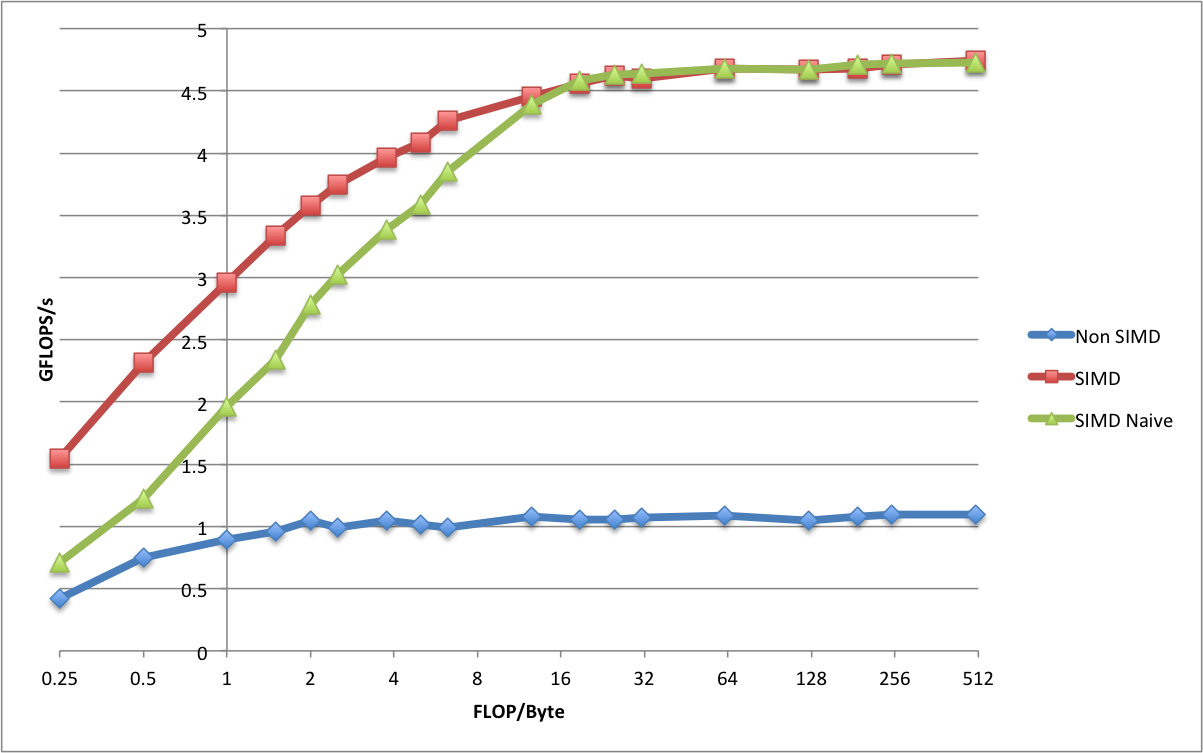
\includegraphics[width=2.5in]{roofline1}
    \caption{Roofline model of hand-tuned JavaScript using both optimized vector loads and naive vector construction}
\end{figure}

The distinction between the "SIMD" and "SIMD Naive" lines is that the "SIMD"
version uses optimized vector load instructions while the "SIMD Naive" version
uses regular vector construction by putting each element of the array into the
vector separately.  As expected, the version using optimized vector loads
outperformed naively constructing the vectors at low computational complexities
while they matched each other at higher complexities where the overhead of
vector construction is much less significant.

In Figure 2 we present the roofline model generated using the same operation as
above but comparing the hand-tuned SIMD implementation to our auto-generated
SIMD implementation.

\begin{figure}[!t]
    \centering
    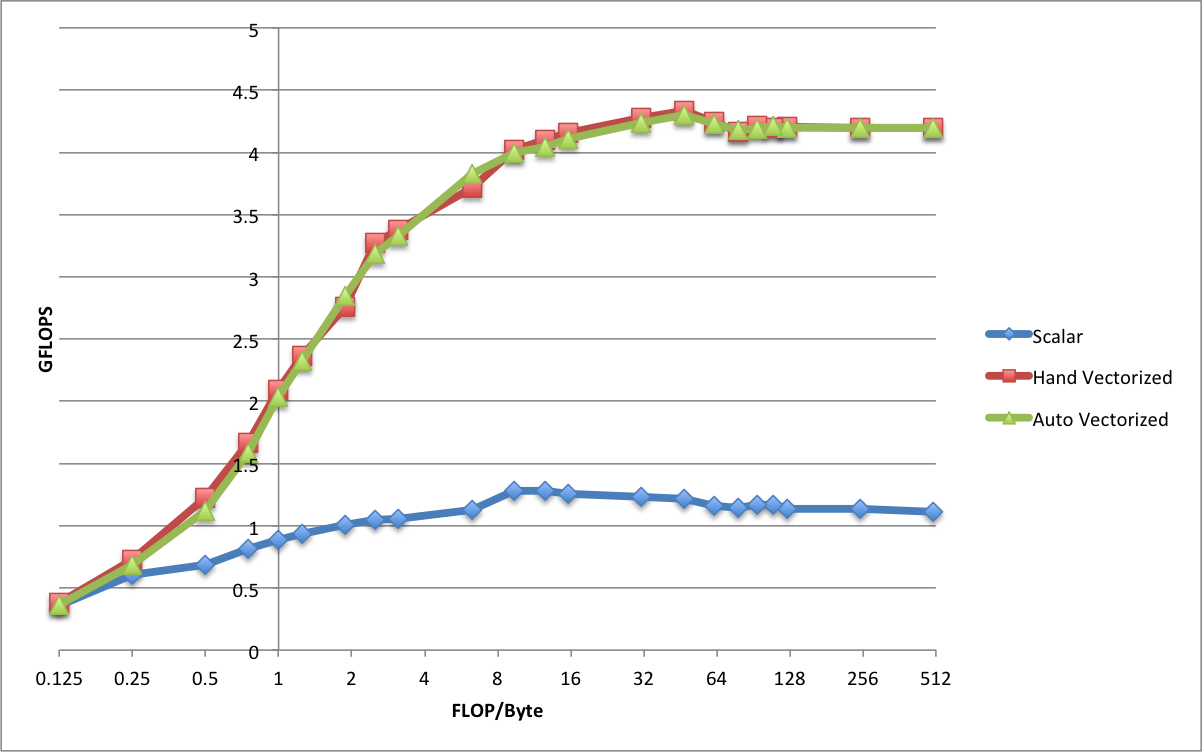
\includegraphics[width=2.5in]{roofline2}
    \caption{Roofline model of auto-generated vector code vs. hand-tuned vector code}
\end{figure}

We see that our auto-generated version produces identical results the hand
written version while requiring no additional effort to create. In both cases
the vectorized version of the code achieved a nearly 4x speedup at approximately
16 operations per byte. This corresponds to 64 operations per float. This is
a very large number for typical JavaScript, but even on loops with as few as
four operations per float, a nearly 2x speedup was observed.

While vectorizing code, there are many things to take into account in terms of
generating efficient code. In JavaScript this is especially true as there many
ways to achieve identical results. In the following sections we describe three
optimizations made while generating code that greatly increased performance on
three selected benchmarks: Map +2, Map Inner Loop 1, and Map Inner Loop 2. Map
+2 simply adds two to every index of an array. This benchmark has very low
computational complexity and gives advantage to the scalar version which will
not incur the overhead of vector construction. Map Inner Loop 1 and 2, by
contrast, have a very high computational complexity and show us how the
JavaScript engine reacts to a tight inner loop adding a constant every
iteration and a tight inner loop adding a variable every iteration.

\subsection{Local Variables}
In order to achieve vectorization, our library generates temporaries to
hold SIMD vectors corresponding to various indices. This allows us to avoid
reading the array multiple times to construct identical vectors. In the first
iteration of our library we assigned directly to these temporaries instead
of declaring them first. This resulted in the JavaScript engine scanning the
current environment for variables of that name to overwrite every time we
created a new temporary. When we observed a nearly 40x slowdown vs. scalar
code we suspected this may be a problem! By converting all temporary assignments
to declare the temporary as local we significantly sped up the code. Table
1 summarizes the gains from this optimization.

\begin{table}[!t]
\centering
\caption{}
\begin{tabular}{|l||c|c|c|c|}
\hline
Benchmark & Scalar & Hand-Tuned & Global & Local \\ \hline
Map +2 & 0.059ms & 0.192ms & 22.133ms & 9.749ms \\ \hline
Map Inner Loop 1 & 8.819ms & 3.798ms & 299.308ms & 13.824ms \\ \hline
Map Inner Loop 2 & 25.319ms & 2.357ms & 389.091ms & 11.714ms \\ \hline
\end{tabular}
\end{table}

\subsection{Index Efficiency}
Our first approach to vectorization was to transform the induction variable
into a vector of four consecutive steps of the induction variable and then
index into the array using the vector accessors. Our code ended up looking like
this:
\begin{verbatim}
for (int i = 0; i + 3 < len; i += 4) {
    var temp_i = vec(i, i+1, i+2, i+3);
    var temp_array = vec(array[temp_i.x],
                         array[temp_i.y],
                         array[temp_i.z],
                         array[temp_i.w]);
    ...
}
\end{verbatim}

While this provided a very clean abstraction in the code, it turned out to be
very inefficient as the round-trip overhead of creating a vector only to
immediately deconstruct it was significant. In our second approach, We ended up
tracking the induction variable separately from other vectors so we could avoid
this overhead. The equivalent code after this optimization became:
\begin{verbatim}
for (int i = 0; i + 3 < len; i += 4) {
    var temp_array = vec(array[i],
                         array[i+1],
                         array[i+2],
                         array[i+3]);
    ...
}
\end{verbatim}

In Table 2 we present results for this optimization. We see in the general case
this optimization reduced our execution time by about 0.8ms howver in the
simple map (+2) operation we reduced our execution time by over 20x. This is
likely due to the javascript engine being able to recognize the loop in the
second case and optimizing much more aggresively.

\begin{table}[!t]
\centering
\caption{}
\begin{tabular}{|l||c|c|c|c|}
\hline
Benchmark & Scalar & Hand-Tuned & Approach 1 & Approach 2 \\ \hline
Map +2 & 0.059ms & 0.192ms & 9.165ms & 0.358ms \\ \hline
Map Inner Loop 1 & 8.819ms & 3.798ms & 13.112ms & 12.307ms \\ \hline
Map Inner Loop 2 & 25.319ms & 2.357ms & 11.189ms & 10.362ms \\ \hline
\end{tabular}
\end{table}


\subsection{Evil Eval}
At the end of our vectorization pipeline, we receive a string from the code
generator containing the vectorized function source. Our first inclination was
to \texttt{eval} this code in order to convert it to JavaScript again. We found
however that even when our optimization was producing identical code to the
hand-tuned versions, it was at an over 3x speed disadvantage. Inspecting the
SpiderMonkey metadata for our generated function we found that it was treating
it as a "Lazy" function and as we suspect, not optimizing it as aggresively as
the non-\texttt{eval}'d functions. In order to mitigate this we converted our
function source to JavaScript functions by using the Function constructor which
we expected to have more standardized results. We found this made a significant
improvement in runtimes such that our auto generated versions performed nearly
identically to the hand-tuned versions.

In Table 3 we present the results of this modification. This optimization
completely closed the gap between the hand-tuned version and the auto-generated
one.

\begin{table}[!t]
\centering
\caption{}
\begin{tabular}{|l||c|c|c|c|}
\hline
Benchmark & Scalar & Hand-Tuned & Eval & Function \\ \hline
Map +2 & 0.059ms & 0.192ms & 0.367ms & 0.197ms \\ \hline
Map Inner Loop 1 & 8.819ms & 3.798ms & 12.489ms & 3.641ms \\ \hline
Map Inner Loop 2 & 25.319ms & 2.357ms & 10.362ms & 2.401ms \\ \hline
\end{tabular}
\end{table}

\section{Surprises}
\section{Lessons Learned}

  One of the most important lessons we picked up on our endeavor was the value
  of an intermediate representation specifically built towards compiler
  optimizations. While working at such a high level does provide certain
  niceties, such as being able to trivially identify loops, there a many more
  burdens that come with it.

  JavaScript is a language with very complicated semantics many of which
  JavaScript developers exploit. These semantics forced us to make a number of
  simplifying assumptions which a production grade compiler should not. For
  example, to safely vectorize loops an important consideration is a pointer
  aliasing. While this problem is challenging and has mostly imperfect
  solutions for languages such as C, Javascript's semantics greatly complicate
  the matter.  Thanks to Javascript's ``variable hoisting'' not only can
  programmers use variables which are not defined in the given scope, they can
  add them to the scope at runtime. As a result, for sake of not embarking on
  an entirely different project, our optimizer makes the assumptions that
  identifiers with distinct names will point to distinct structures.

  Moreover, the fact that JavaScript is dynamically typed and overloads all
  infix operators makes it virtually impossible to determine whether a given
  expression will always evaluate to a floating point value without performing
  some sort of interprocedural analysis. Take the following as an example,
  \begin{verbatim}
    function foo (var arg) {
      for (var i = 0; i < 5; i++) {
        arg[i] += 1;
      }
      return arg;
    }
  \end{verbatim}
  If a user were to call $\texttt{foo([1, 2])}$ we could safely vectorize the
  funciton, but if the users uses it as $\texttt{foo(['bar', 'baz'])}$ we could
  not, even though they both are valid uses of the function.

  It's resoundingly clear that to build a production grade version of our tool
  a significant portion of time would have to be allocated dealing with the
  intricacies of JavaScript. In retrospect at the onset of our development we
  should have clearly outlined not only the features of JavaScript which we
  were support, but those we were ignoring them.



% needed in second column of first page if using \IEEEpubid
%\IEEEpubidadjcol

% An example of a floating figure using the graphicx package.
% Note that \label must occur AFTER (or within) \caption.
% For figures, \caption should occur after the \includegraphics.
% Note that IEEEtran v1.7 and later has special internal code that
% is designed to preserve the operation of \label within \caption
% even when the captionsoff option is in effect. However, because
% of issues like this, it may be the safest practice to put all your
% \label just after \caption rather than within \caption{}.
%
% Reminder: the "draftcls" or "draftclsnofoot", not "draft", class
% option should be used if it is desired that the figures are to be
% displayed while in draft mode.
%
%\begin{figure}[!t]
%\centering
%\includegraphics[width=2.5in]{myfigure}
% where an .eps filename suffix will be assumed under latex,
% and a .pdf suffix will be assumed for pdflatex; or what has been declared
% via \DeclareGraphicsExtensions.
%\caption{Simulation Results}
%\label{fig_sim}
%\end{figure}

% Note that IEEE typically puts floats only at the top, even when this
% results in a large percentage of a column being occupied by floats.


% An example of a double column floating figure using two subfigures.
% (The subfig.sty package must be loaded for this to work.)
% The subfigure \label commands are set within each subfloat command, the
% \label for the overall figure must come after \caption.
% \hfil must be used as a separator to get equal spacing.
% The subfigure.sty package works much the same way, except \subfigure is
% used instead of \subfloat.
%
%\begin{figure*}[!t]
%\centerline{\subfloat[Case I]\includegraphics[width=2.5in]{subfigcase1}%
%\label{fig_first_case}}
%\hfil
%\subfloat[Case II]{\includegraphics[width=2.5in]{subfigcase2}%
%\label{fig_second_case}}}
%\caption{Simulation results}
%\label{fig_sim}
%\end{figure*}
%
% Note that often IEEE papers with subfigures do not employ subfigure
% captions (using the optional argument to \subfloat), but instead will
% reference/describe all of them (a), (b), etc., within the main caption.


% An example of a floating table. Note that, for IEEE style tables, the
% \caption command should come BEFORE the table. Table text will default to
% \footnotesize as IEEE normally uses this smaller font for tables.
% The \label must come after \caption as always.
%
%\begin{table}[!t]
%% increase table row spacing, adjust to taste
%\renewcommand{\arraystretch}{1.3}
% if using array.sty, it might be a good idea to tweak the value of
% \extrarowheight as needed to properly center the text within the cells
%\caption{An Example of a Table}
%\label{table_example}
%\centering
%% Some packages, such as MDW tools, offer better commands for making tables
%% than the plain LaTeX2e tabular which is used here.
%\begin{tabular}{|c||c|}
%\hline
%One & Two\\
%\hline
%Three & Four\\
%\hline
%\end{tabular}
%\end{table}

 % TAG  SOURCE
 % CIT0 https://hacks.mozilla.org/2014/10/introducing-simd-js/
%\bibitem{IEEEhowto:kopka}
%H.~Kopka and P.~W. Daly, \emph{A Guide to \LaTeX}, 3rd~ed.\hskip 1em plus
% 0.5em minus 0.4em\relax Harlow, England: Addison-Wesley, 1999.
%\end{thebibliography}


% Note that IEEE does not put floats in the very first column - or typically
% anywhere on the first page for that matter. Also, in-text middle ("here")
% positioning is not used. Most IEEE journals use top floats exclusively.
% Note that, LaTeX2e, unlike IEEE journals, places footnotes above bottom
% floats. This can be corrected via the \fnbelowfloat command of the
% stfloats package.

% if have a single appendix:
%\appendix[Proof of the Zonklar Equations]
% or
%\appendix  % for no appendix heading
% do not use \section anymore after \appendix, only \section*
% is possibly needed

% use appendices with more than one appendix
% then use \section to start each appendix
% you must declare a \section before using any
% \subsection or using \label (\appendices by itself
% starts a section numbered zero.)
%

% use section* for acknowledgement
\section*{Acknowledgment}


The authors would like to thank...


% Can use something like this to put references on a page
% by themselves when using endfloat and the captionsoff option.
\ifCLASSOPTIONcaptionsoff
  \newpage
\fi

% trigger a \newpage just before the given reference
% number - used to balance the columns on the last page
% adjust value as needed - may need to be readjusted if
% the document is modified later
%\IEEEtriggeratref{8}
% The "triggered" command can be changed if desired:
%\IEEEtriggercmd{\enlargethispage{-5in}}

% references section

% that's all folks
\end{document}
